This chapter describes the method proposed in this work for evaluating assistive devices using virtual reality. The method is organized into 5 phases as illustrated in Figure \ref{fig:diag_metodologia}.


%\tikzstyle{start} = [rectangle, rounded corners, minimum width=4cm, minimum height=1.0cm,text centered, draw=black, fill=white!30, text width=3cm]
\tikzstyle{process} = [rectangle, minimum width=4cm, minimum height=1.0cm, text centered, draw=black, fill=white!30, text width=3.5cm]
\tikzstyle{decision} = [diamond, minimum width=3.5cm, minimum height=1.0cm,  text centered, text width=3.5cm, draw=black, fill=white!30]
\tikzstyle{arrow_flow} = [ccmDBlue, rounded corners, line width = 2mm, ->]
\tikzstyle{arrow_return} = [ccmRed, rounded corners, line width = 2mm, ->]

\begin{tikzpicture}[node distance=2cm]
    \centering
    \node (start) [start] {Collect the ECG Data};
    \node (read) [process, below of=start,yshift=-0.5cm] {Read the GSR file};
    \node (average) [process, aspect=2.5, below of=read, yshift=-0.5cm] {Calculate the average};
    %\node (std) [process, aspect=2.5, below of=average, yshift=-0.5cm] {Calculate the standard deviaton};
    
    \draw [arrow_flow] (start.south) -- (read.north);
    \draw [arrow_flow] (read.south) -- (average.north);
    %\draw [arrow_flow] (average.south) -- (std.north);
    %\draw [arrow_flow] (std.south) -- (findPeaks.north);
    
\end{tikzpicture}
\begin{figure*}[!htb]
    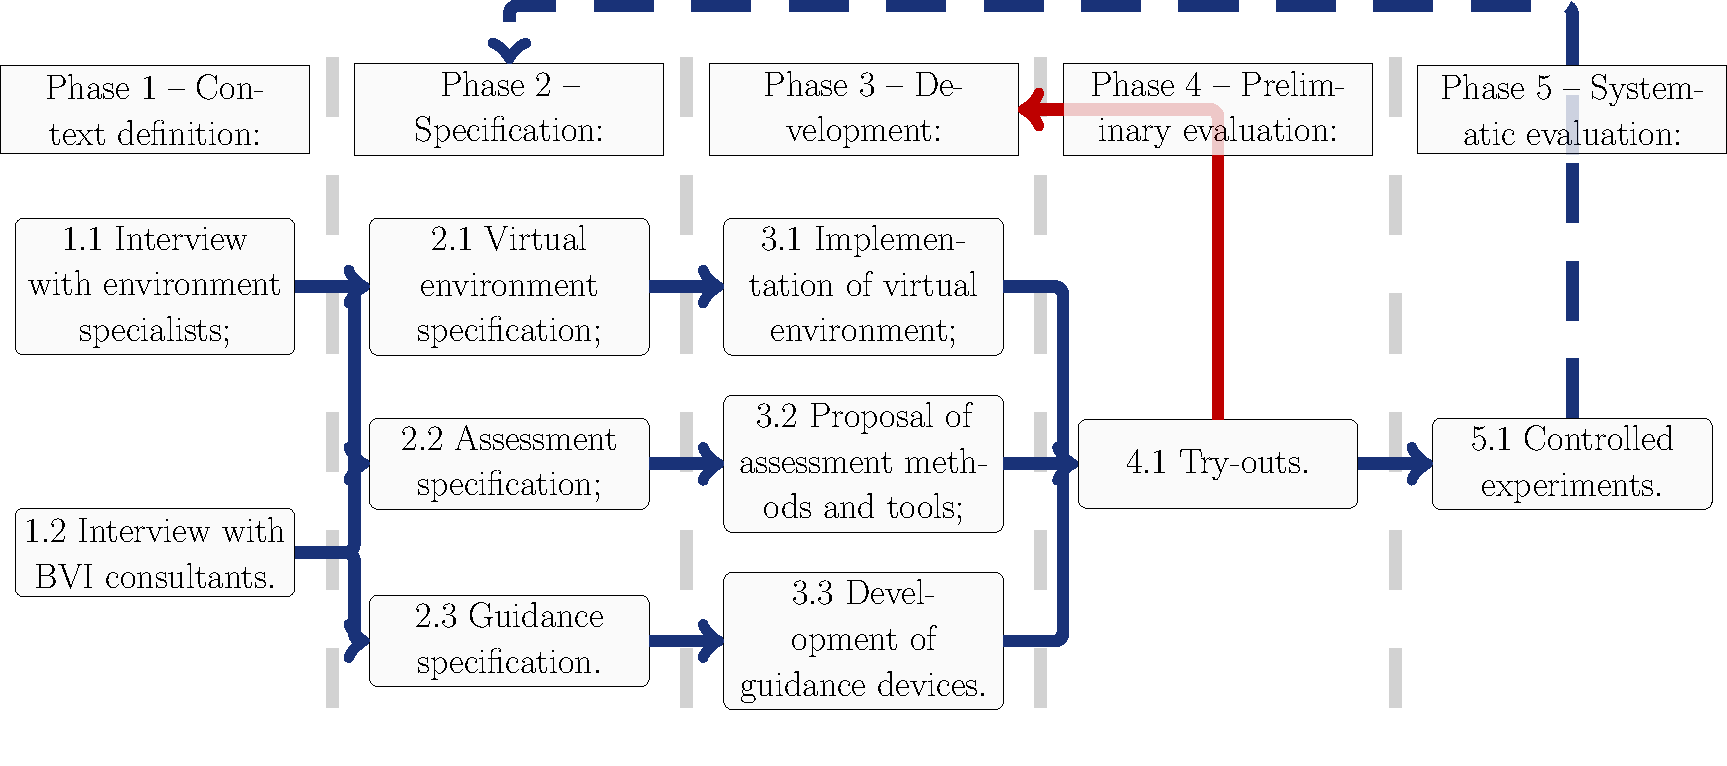
\includegraphics[width = \linewidth]{2 - Metodologia/metodologia.pdf}
    \caption{Method's diagram}
    \label{fig:diag_metodologia}
\end{figure*}

%% ---------------------------
%% 1 Phase
%% ---------------------------

The first phase is the context definition. It consists of defining the main features of the environment in which the assistive device will be used, based on interviews from hospital's specialists from São José dos Campos. It also includes a step for understanding the limitations of the current assistive devices and defining the main features of assistive devices to be designed. This last step is based on interviews with two BVI users, one that is blind since 13 years old and another that has Usher's disease.

%% ---------------------------
%% 2 Phase
%% ---------------------------

In the second phase, the information collected through the interviews of Phase 1 is used to make critical decisions about the virtual environment where the evaluation of the assistive devices will be carried out. It is also used to define which human factors should be assessed. Finally, it contributes to define the guidance devices that should be implemented in the assistive devices.

%% ---------------------------
%% 3 Phase
%% ---------------------------

    The third phase is dedicated to developing the virtual environment, the evaluation tools and techniques, and the first proof of concept of the assistive devices, which should be integrated into the virtual environment for testing.

    %% ---------------------------
    %% Virtual Environment
    %% ---------------------------
    \subsection*{Virtual Environment}
    The virtual reality environment was developed using the Unity3D platform and the implementation should be followed by preparing the corresponding physical space to perform the test campaign. Following the recommendations from the BVI interviews, typical reception furniture was placed in the virtual environment as illustrated in Figure \ref{fig:task_diagram}. Sounds were also used to increase the feeling of immersion and indicate to the BVI participant where the reception desk was located. The participant navigation through the reception was composed of 4 tasks, also illustrated in Figure \ref{fig:task_diagram}:

    \begin{enumerate}
        \item Clean the hands at the sanitizer totem (COVID-19 procedures);
        \item Go to the reception desk to receive a queue number;
        \item Go to the waiting area and wait for the number calling;
        \item Leave the room when called.
    \end{enumerate}

    \begin{figure}[!htb]
        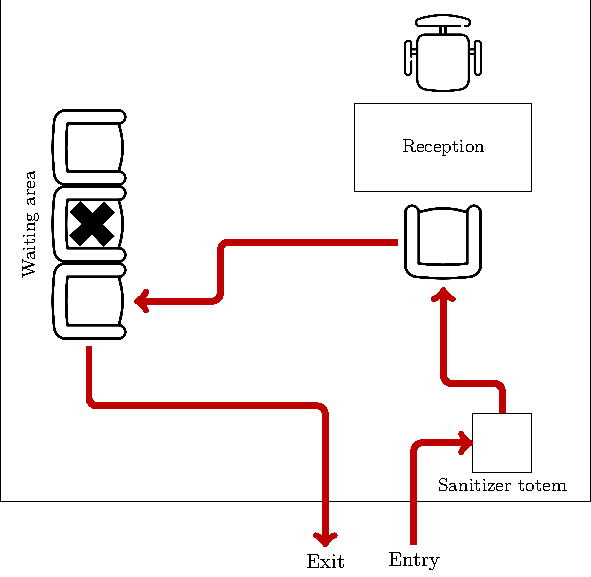
\includegraphics[width = \linewidth]{2 - Metodologia/caminho.pdf}
        \caption{Scheduled task of the experiment and their order.}
        \label{fig:task_diagram}
    \end{figure}

    Figure \ref{fig:ve_phot} shows the virtual environment created in Unity3D and the corresponding real environment assembled at the CCM entrance hall. 

    \begin{figure}[!htb]
        \centering
        \begin{subfigure}[b]{0.75\linewidth}
            \centering
            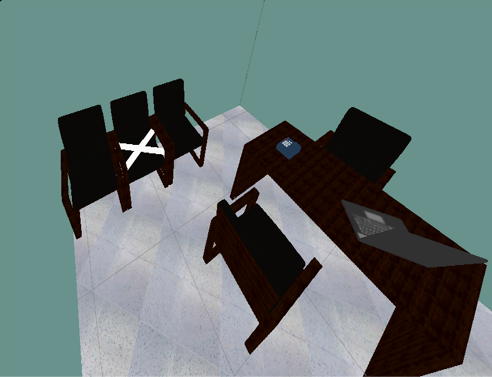
\includegraphics[width=\linewidth]{2 - Metodologia/VE.png}
            \caption{Virtual environment screenshot}
            \label{fig:ve_photo}
        \end{subfigure}
        \hfill
        \begin{subfigure}[b]{0.75\linewidth}
    %\end{figure}    
    %\begin{figure}[!htb]
            \centering
            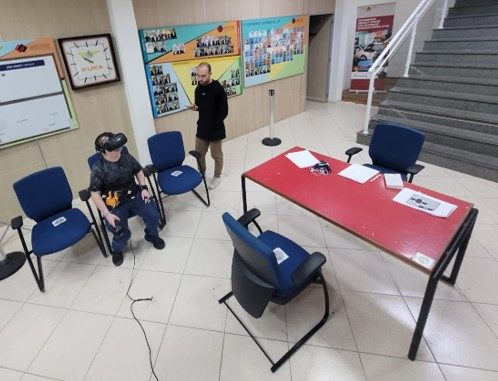
\includegraphics[width=\linewidth]{2 - Metodologia/RE.jpg}
            \caption{   }
            \label{fig:re_photo}
        \end{subfigure}
        \caption{Environment comparisson}
        \label{fig:ve_re}
    \end{figure}


    %% ---------------------------
    %% Human Factors techniques
    %% ---------------------------
    \subsection*{Human Factors techniques}
    The assessment should evaluate workload, situation awareness and the user's impressions using:

%\begin{enumerate} [label = \Alph*)]
%    \item Task Performance;
%\end{enumerate}
%    
%In the hospital reception scenario, the proposed measurement related to BVI performance is the number of times the BVI user hits the furniture in the virtual environment during the tasks' execution.

    \begin{enumerate} [1.]
        \setcounter{enumi}{0}
        \item Workload;
    \end{enumerate}

    Following the recommendations from the review of literature, the workload is estimated using two approaches:
    \begin{itemize}
        \item Physiological measures obtained from an ECG (Electrocardiogram) sensor and a GSR (Galvanic Skin Response) sensor;
        \item NASA-TLX (National Aeronautics and Space Administration Task Load Index) subjective questionnaire.
    \end{itemize}

    \begin{enumerate} [2.]
        \setcounter{enumi}{1}
        \item Situation awareness;
    \end{enumerate}

    A modified SAGAT (Situation Awareness Global Assessment Technique) questionnaire is used to evaluate the BVI situation awareness.
    As original idea from \cite{endsley1988design}, the proposed version is based on 3 levels of situation awareness:
    
    \begin{enumerate}[Level 1.]%[leftmargin = 6em, label = Level \arabic* -- ]
        \item Perception
        
        It aims to evaluate if the user can perceive the environment surrounding him/her.

        \item Comprehension

        After the user answer about an detected object, he/she is asked to point to where the object is located. 

        \item Projection
        
        This level is measured after every question that asks the location of an object. He/she is then required to answer how far he/she supposes that this object is
        
    \end{enumerate}      

    \begin{enumerate} [3.]
        \setcounter{enumi}{2}
        \item Devices evaluation;
    \end{enumerate}

    Finally, a questionnaire is proposed for evaluating the guidance devices. The questions were about the comfort, the sense of safety, the sense of confusion and on the precision that the manipulation of the device caused.

    %% ---------------------------
    %% Assistive Devices
    %% ---------------------------
    \subsection*{Assistive Devices}
    Four guidance methods were proposed to be evaluated in this work.
        
    \begin{enumerate} [1.]
        \item Audio guidance;
        
        The first method is audio guidance. Basically, in the course of the experiment, the participant could give two different voice commands: “What is around me?” and “Where is (something)?”. The answers of both commands was done with the interference of a member of the design team.  

        \item Vibration guidance with command – virtual cane;
        
        When using a white cane, the user points it to check nearby obstacles in a specific direction. The virtual cane has a similar way of functioning, but instead of connecting the user to the nearby object through the cane, it vibrates when it detects an obstacle in the direction the user pointed it.

        \item Vibration guidance without command – haptic belt
        
        The belt has appended 8 vibration units that vibrate accordingly to the direction and distance of the closest object around the user. The main differences between the virtual cane and the haptic belt is that the haptic belt checks 360° around the user. When objects are within a certain limit, it vibrates indicating to the user the direction of the closest object. 

        \item Mixture of audio and vibration guidance
        
        This option is implemented making the three options available to the user: audio guidance, haptic belt and virtual cane. 
    \end{enumerate}


The fourth phase provides a preliminary assessment of the devices through its unstructured experimentation by BVI consults. This preliminary assessment provides feedback for improving the device concept. The cycle of “try-out and improve device concept” can be repeated until the device concept is considered mature to be tested through a systematic set of controlled experiments.

The fifth phase consists of executing a campaign of controlled experiments, following the best practices of the DoE (Design of Experiments) discipline, and analysing the results. Concluded this phase, the results should provide information for the design team to decide between proceeding to the detailed design of the assistive devices or performing a new evaluation cycle.

In the case of this work, the proposed experiment consists of asking the participant to use five guidance methods: the audio guidance, haptic belt, virtual cane, mixed and, additionally, the device used daily by the BVI (e.g., white cane). Moreover, each participant should use each guidance method twice (“first visit” and “return visit”), in order to provide some information about how the guidance devices performs in new and known environments. In order to avoid the learning effect from one method to the other, five versions of the reception scene are developed, changing the position of the objects - one version to be used with each guidance method. The scene order is randomized for each participant.

Moreover, particularly in the case of this work, an additional round of tests is added to the experiment to investigate the differences between the evaluation performed by BVI users and sighted (non-BVI) users. For this purpose, the same experiment is repeated with a set of non-BVI users. The purpose is to investigate whether or not performing the analysis with non-BVI users could lead to different conclusions.

The experiment is organized in the following way:

\begin{itemize}
    \item Briefing:
    \item Execution of the experiment:
    \begin{itemize}
        \item Guidance method training;
        \item First visit and SAGAT questionnaire;
        \item NASA-TLX for the first visit;
        \item Return visit and SAGAT questionnaire;
        \item NASA-TLX for the return visit;
        \item Questionnaire about the guidance method.
    \end{itemize}
    \item Experiment's conclusion
\end{itemize}

As a result of the experiment, the following data are collected:

\begin{itemize}
    \item Answers to the NASA-TLX questionnaire;
    \item ECG and GSR signals;
    \item Answers to the SAGAT questionnaire;
    \item Answers to the guidance method questionnaire.
\end{itemize}